\chapter{Métodos dos Elementos Finitos}\label{cap:elementosfinitos}

O MEF é uma ferramenta de simulação empregada em diversos campos da engenharia, sendo utilizada desde a análise de sólidos e estruturas à transferência de calor e fluidos \cite{bathe2006finite}. 

Como existe uma gama de materiais publicados sobre esse tema, este capítulo irá apresentá-lo resumidamente, de modo a possibilitar a compreensão do trabalho realizado no capítulo 5. Para um aprofundamento sobre o MEF, \cite{bathe2006finite}, \cite{felippa2004introduction} e \cite{felippa2003advanced} são leituras recomendadas.

Na análise pelo MEF,uma aproximação da variável de interesse é definida, por meio de funções de interpolação dos valores incógnitos dessas variáveis, posteriormente, a estrutura é discretizada como sendo composta por elementos finitos, formados por arestas conectadas a vértices por meio de nós. Um sistema de equações discretas é obtido e após aplicar condições de contorno, os valores das variáveis de interesse são obtidos e o comportamento geral da estrutura foi então simulado/aproximado.

Desse modo, para simular o comportamento do material acolchoado durante o impacto no teste de queda, mostrado na figura \ref{fig:CorpoDeProva}, é realizado uma subdivisão desse material em elementos tetraédricos, sendo cada um formado por 4 nós. A malha resultante é mostrada na figura \ref{fig:ElementoFinito}. 

 \begin{figure}[H]  
        \centering
        \caption{Corpo de prova com material acolchoado.}
        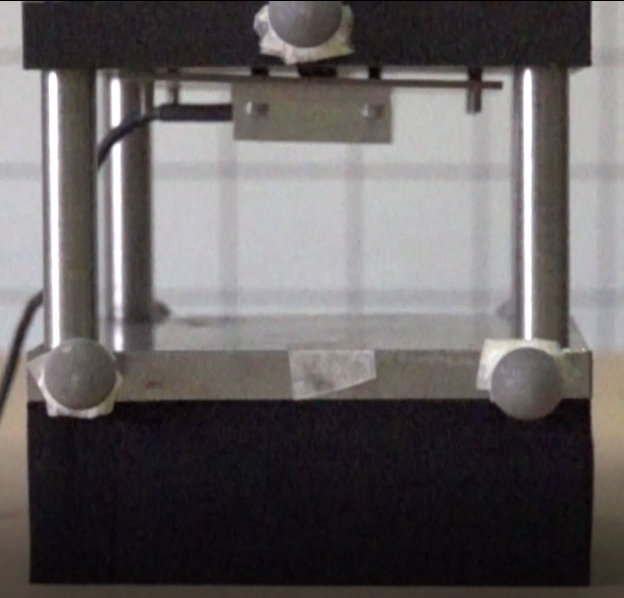
\includegraphics[width=8cm]{./figs/CorpoDeProva.PNG}
        \par\medskip
        Fonte: Própria autoria.
        \label{fig:CorpoDeProva}
\end{figure}

 \begin{figure}[H]  
        \centering
        \caption{Material acolchoado sendo modelado por uma malha tetraédrica.}
        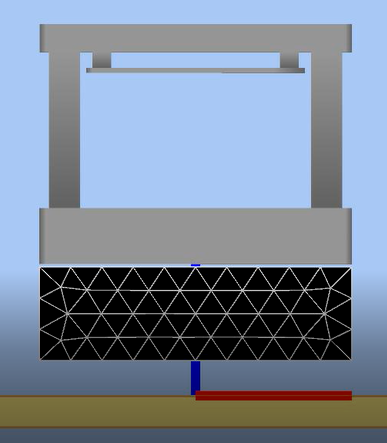
\includegraphics[width=8cm]{./figs/MaterialDividido.PNG}
        \par\medskip
        Fonte: Própria autoria.
        \label{fig:ElementoFinito}
\end{figure}


Conforme \cite{Chen2017numerical}, para o elemento tetraédrico, mostrado na figura \ref{fig:finiteelement}, as coordenadas e deslocamentos, medidos nas coordenadas locais, dos nós 1, 2, 3 e 4 são, respectivamente, $(x_{i}, y_{i}, z_{i})$ e $(u_{i}, v_{i}, w_{i})$, para $i = {1, 2, 3, 4}$.

 A função de otimização que determina o deslocamento $(u, v, w)$ do ponto $(x, y, z)$ é expressa da seguinte maneira:
 
 %funcao de interpolacao linear
 
 \begin{figure}[h]  
        \centering
        \caption{Deslocamento dos nós para um elemento tetraédrico. \cite{Chen2017numerical}.}
        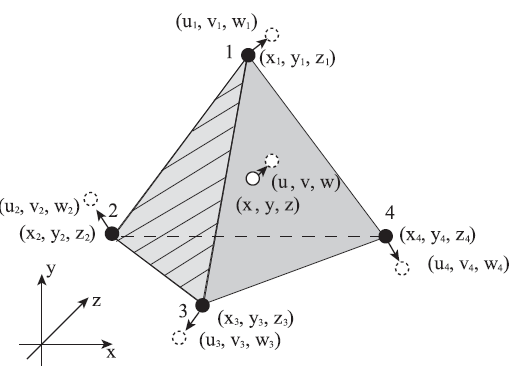
\includegraphics[width=8cm]{./figs/finiteelement.png}
        \label{fig:finiteelement}
\end{figure}

\begin{equation}
\label{eqn:interpolation}
\begin{aligned}
u &= \alpha_{1} + \alpha_{2}x + \alpha_{3}y + \alpha_{4}z, \\
v &= \alpha_{5} + \alpha_{6}x + \alpha_{7}y + \alpha_{8}z, \\
w &= \alpha_{9} + \alpha_{10}x + \alpha_{11}y + \alpha_{12}z
\end{aligned}
\end{equation}

Neste trabalho, o material estudado é considerado isotrópico, homogêneo e com deformação linear. Sob essas hipóteses, as deformações de engenharia $\epsilon_{e} = (\epsilon_{x}, \epsilon_{y}, \epsilon_{z}, \gamma_{xy}, \gamma_{yz}, \gamma_{zx})$, são definidas da seguinte forma:

\begin{equation} \label{eq:axialdef}
    \begin{aligned}
    &\epsilon_{x} = \frac{\partial u}{\partial x}, 
    &\epsilon_{y} = \frac{\partial v}{\partial y}, 
    &\epsilon_{z} = \frac{\partial w}{\partial z}
    \end{aligned}
\end{equation}

\begin{equation} \label{eq:angulardef}
    \begin{aligned}
    &\gamma_{xy} = \frac{\partial u}{\partial y} + \frac{\partial v}{\partial x}, 
    &\gamma_{yz} = \frac{\partial v}{\partial z} + \frac{\partial w}{\partial y}, 
    &\gamma_{zx} = \frac{\partial w}{\partial x} + \frac{\partial u}{\partial z}
    \end{aligned}
\end{equation}

Por meio da Lei de Hooke, as deformações podem ser reescritas da seguinte forma:

\begin{equation} \label{eq:tensaodeformacao1}
    \begin{aligned}
        \epsilon_{x} = \frac{\sigma_{x} - \nu(\sigma_{y} + \sigma_{z})}{E},
        \epsilon_{y} = \frac{\sigma_{y} - \nu(\sigma_{z} + \sigma_{x})}{E},
        \epsilon_{z} = \frac{\sigma_{z} - \nu(\sigma_{x} + \sigma_{y})}{E}
    \end{aligned}    
\end{equation}
\begin{equation} \label{eq:tensaodeformacao2}
    \begin{aligned}
        \gamma_{xy} = \frac{\uptau_{xy}}{G},
        \gamma_{yz} = \frac{\uptau_{yz}}{G},
        \gamma_{zx} = \frac{\uptau_{zx}}{G}
    \end{aligned}
\end{equation}
onde $E$, $G$ e $\nu$ são, respectivamente, Módulo de Young, Módulo de Cisalhamento e Coeficiente de Poisson.

Das equações \ref{eqn:interpolation}, \ref{eq:axialdef} e \ref{eq:angulardef}, \ref{eq:tensaodeformacao1} e \ref{eq:tensaodeformacao2} obtêm-se as seguintes relações matriciais:

\begin{equation} \label{eq:matrixdisplacement}
    \begin{Bmatrix}
        u_{1} \\
        v_{1} \\
        w_{1} \\
        u_{2} \\
        v_{2} \\
        w_{2} \\
        u_{3} \\
        v_{3} \\
        w_{3} \\
        u_{4} \\
        v_{4} \\
        w_{4} \\
    \end{Bmatrix}
    = 
    \begin{bmatrix}
    1 & x_{1} & y_{1} & z_{1} & 0 & 0 & 0 & 0 & 0 & 0 & 0 & 0 \\
    0 & 0 & 0 & 0 &  1 & x_{1} & y_{1} & z_{1} & 0 & 0 & 0 & 0 \\
    0 & 0 & 0 & 0 & 0 & 0 & 0 & 0 & 1 & x_{1} & y_{1} & z_{1} \\
    1 & x_{2} & y_{2} & z_{2} & 0 & 0 & 0 & 0 & 0 & 0 & 0 & 0 \\
    0 & 0 & 0 & 0 &  1 & x_{2} & y_{2} & z_{2} & 0 & 0 & 0 & 0 \\
    0 & 0 & 0 & 0 & 0 & 0 & 0 & 0 & 1 & x_{2} & y_{2} & z_{2} \\
    1 & x_{3} & y_{3} & z_{3} & 0 & 0 & 0 & 0 & 0 & 0 & 0 & 0 \\
    0 & 0 & 0 & 0 &  1 & x_{3} & y_{3} & z_{3} & 0 & 0 & 0 & 0 \\
    0 & 0 & 0 & 0 & 0 & 0 & 0 & 0 & 1 & x_{3} & y_{3} & z_{3} \\
    1 & x_{4} & y_{4} & z_{4} & 0 & 0 & 0 & 0 & 0 & 0 & 0 & 0 \\
    0 & 0 & 0 & 0 &  1 & x_{4} & y_{4} & z_{4} & 0 & 0 & 0 & 0 \\
    0 & 0 & 0 & 0 & 0 & 0 & 0 & 0 & 1 & x_{4} & y_{4} & z_{4} \\
    \end{bmatrix}
    \begin{Bmatrix}
        \alpha_{1} \\
        \alpha_{2} \\
        \alpha_{3} \\
        \alpha_{4} \\
        \alpha_{5} \\
        \alpha_{6} \\
        \alpha_{7} \\
        \alpha_{8} \\
        \alpha_{9} \\
        \alpha_{10} \\
        \alpha_{11} \\
        \alpha_{12} \\
    \end{Bmatrix}
\end{equation}

\begin{equation} \label{eq:matrixalphadisplacement}
    \begin{Bmatrix}
        \epsilon_{x} \\
        \epsilon_{y} \\
        \epsilon_{z} \\
        \gamma_{xy} \\
        \gamma_{yz} \\
        \gamma_{zx} \\
    \end{Bmatrix}
    = 
    \begin{bmatrix}
    0 & 1 & 0 & 0 & 0 & 0 & 0 & 0 & 0 & 0 & 0 & 0 \\
    0 & 0 & 0 & 0 & 0 & 0 & 1 & 0 & 0 & 0 & 0 & 0 \\
    0 & 0 & 0 & 0 & 0 & 0 & 0 & 0 & 0 & 0 & 0 & 1 \\
    0 & 0 & 1 & 0 & 0 & 1 & 0 & 0 & 0 & 0 & 0 & 0 \\
    0 & 0 & 0 & 0 & 0 & 0 & 0 & 1 & 0 & 0 & 1 & 0 \\
    0 & 0 & 0 & 1 & 0 & 0 & 0 & 0 & 0 & 1 & 0 & 0 \\
    \end{bmatrix}
    \begin{Bmatrix}
        \alpha_{1} \\
        \alpha_{2} \\
        \alpha_{3} \\
        \vdots \\
        \alpha_{11} \\
        \alpha_{12} \\
    \end{Bmatrix}
\end{equation}

\begin{equation} \label{eq:elasticitymatrix}
    \begin{Bmatrix}
        \sigma_{x} \\
        \sigma_{y} \\
        \sigma_{z} \\
        \uptau_{xy} \\
        \uptau_{yz} \\
        \uptau_{zx} \\
    \end{Bmatrix} 
    =
    \frac{E(1 - \nu)}{(1+\nu)(1 - 2\nu)}
    \begin{bmatrix}
        1 & \frac{\nu}{1-\nu} & \frac{\nu}{1-\nu} & 0 & 0 & 0 \\
        \frac{\nu}{1-\nu} & 1 & \frac{\nu}{1-\nu} & 0 & 0 & 0 \\
        \frac{\nu}{1-\nu} & \frac{\nu}{1-\nu} & 1 & 0 & 0 & 0 \\
        0 & 0 & 0 & \frac{1-2\nu}{2(1-\nu)} & 0 & 0 \\
        0 & 0 & 0 & 0 & \frac{1-2\nu}{2(1-\nu)} & 0 \\
        0 & 0 & 0 & 0 & 0 & \frac{1-2\nu}{2(1-\nu)} \\
    \end{bmatrix}
    
    \begin{Bmatrix}
        \epsilon_{x}\\
        \epsilon_{y}\\
        \epsilon_{z}\\
        \gamma_{xy}\\
        \gamma_{yz}\\
        \gamma_{zx}\\
    \end{Bmatrix}
\end{equation}

Na forma compacta, tem-se, respectivamente,

\begin{equation} \label{eq:simplifiedeq}
    \begin{aligned}
      \pmb{u_{e}} &= \pmb{A}\alpha, \\
      \epsilon_{e} &= \pmb{B}\alpha, \\
      \pmb{\delta_{e}} &= \pmb{C}_{e} \epsilon_{e}
    \end{aligned}
\end{equation}
onde $\pmb{A}$ é a matriz dos coeficientes de deslocamento dos nós e
$\pmb{C}_{e}$ é a matriz de elasticidade. A matriz $B_{e}$, chamada de matriz de tensão-deformação, é definida como $\pmb{B}_e = \pmb{B}\pmb{A}^{-1}$.

Do princípio do trabalho virtual, a matriz de rigidez de um elemento,  $\pmb{K}_{e}$, é definido como:

\begin{equation} \label{eq:elementrig}
    \pmb{K}_{e} = \pmb{B}^{T}_{e}\pmb{C}_{e}\pmb{B}_{e}V_{e} 
\end{equation}
onde $\pmb{C}_{e}$ e $\pmb{B}_{e}$ são as matrizes definidas previamente, e $V_{e}$ é o volume do elemento finito. Para um elemento tetraédrico, o volume depende das coordenadas dos 4 nós e é dado por:

\begin{equation} \label{eq:volume}
V_{e} = \frac{1}{6} 
\begin{vmatrix}
 1 & 1 & 1 & 1 \\
 x1 & x2 & x3 & x4 \\
 y1 & y2 & y3 & y4 \\
 z1 & z2 & z3 & z4 
\end{vmatrix}
\end{equation}

A partir da matriz de rigidez de cada elemento $\pmb{K}_{e}$, a matriz de rigidez global da estrutura, $\pmb{K}$ é calculada.

Para maior detalhamento das deduções realizadas neste capítulo, consultar \cite{Chen2017numerical}.

Na análise dinâmica de estruturas, equação que governa o deslocamento dos $N$ nós de uma malha, conforme \cite{hughes2012finite}, é dada por:

\begin{equation} \label{eq:dynamic}
\pmb{M}\ddot{\pmb{u}} + \pmb{D}\dot{\pmb{u}} + \pmb{K}\pmb{u} = \pmb{f} 
\end{equation}
onde $u$ é o vetor de deslocamento de ordem $N$, $\dot{u}$ e $\ddot{u}$ são, respectivamente, a primeira e segunda derivadas temporais de $u$.

$\pmb{K}$ representa a matriz de rigidez global da estrutura, descrita previamente.

$\pmb{M}$ representa a matriz de massa da estrutura. 
Diversos métodos podem ser utilizados no cálculo da matriz de massa, entretanto dois métodos se destacam, sendo amplamente citados na literatura: a matriz de massa consistente ("Consistent Mass Matrix")  e a matriz de massa concentrada ("Lumped Mass Matrix") \cite{felippa2004introduction}.

%Explicar Consistent Mass Matrix

%Explicar Lumped Mass Matrix

O MEF é um método numérico, assim as soluções obtidas apresentam um erro e sua magnitude depende de alguns fatores. Por exemplo, como a análise de um objeto contínuo é feita por meio de um modelo discreto, a magnitude do erro é influenciada pelo formato do elemento finito ou do nível de refinamento da malha. Ao se utilizar elementos finitos cada vez menores, o MEF tende a soluções mais próximas da solução exata, quando existem, entretanto, aumenta-se o custo computacional envolvido. 
A utilização da matriz de massa concentrada é interessante pois a matriz de massa resultante é diagonal, o que simplifica o custo-computacional envolvido no cálculo de sua inversa, $\pmb{M}^{-1}$.
Por outro lado, a matriz de massa consistente apresenta resultados mais precisos. Entretanto, o tamanho dos elementos escolhido deve ser pequeno, elevando o custo computacional envolvido \cite{Chen2017numerical}.

Para este trabalho, a matriz de massa concentrada é utilizada, uma vez que a malha escolhida não possui elementos finitos pequenos o suficiente que torne o resultado com a matriz de massa consistente mais preciso do que a matriz de massa concentrada. Além disso, a matriz de massa concentrada destaca-se pela relativa simplicidade de aplicação e menor custo-computacional envolvido.

A matriz de massa concentrada $\pmb{M}$, conforme \cite{Chen2017numerical}, é definida como:

\begin{equation} \label{eq:massmatrix}
    \pmb{M} = 
    \begin{pmatrix}
    \pmb{m}_{1} &        &   &    &  \\
                & \ddots &   &  0 &  \\
                &        & \pmb{m}_{i} & & \\
                & 0      &             &  \ddots &\\
                & & & & \pmb{m}_{n}
    \end{pmatrix}
\end{equation}

\begin{equation} \label{eq:mass}
\pmb{m}_{i} =
\begin{pmatrix}
    m_{i} & 0 & 0 \\
    0 & m_{i} & 0 \\
    0 & 0 & m_{i} \\
\end{pmatrix}
\end{equation}
\begin{equation}
    m_{i} = \sum_{j=1}^{N_{ij}} \frac{\rho V_{j}}{4}    
\end{equation}
onde $m_{i}$ é a massa concentrada nó, $\rho$ é a densidade e $V_{j}$ o volume do elemento $j$. $N_{ij}$ é o número de elementos que compartilhar o nó $j$.

$\pmb{D}$ representa a matriz de amortecimento. O amortecimento é utilizado para caracterizar a energia dissipada pelo material acolchoado durante o impacto de queda \cite{ge2018impact}. Será utilizado um modelo viscoso linear, no qual a força de amortecimento é proporcional linearmente à velocidade de deformação. 

Para sistemas de múltiplos graus de liberdade, a teoria de amortecimento ainda não é bem estabelecida. Uma das razões reside na dificuldade em se obter informações sobre o amortecimento de um sistema para o calculo da matriz $\pmb{D}$ \cite{liu1995formulation}.
Uma aproximação comumente aplicada é o amortecimento de Rayleigh, definido como:

\begin{equation} \label{eq:damping}
\pmb{D} = \alpha \pmb{M} + \beta \pmb{K}
\end{equation}
onde $\pmb{M}$ e $\pmb{K}$ são, respectivamente, as matrizes de massa e rigidez, $\alpha$ e $\beta$ são os parâmetros de Rayleigh, constantes arbitrárias obtidas experimentalmente, pois variam de acordo com o design da estrutura e o material aplicado. Além disso, esses parâmetros não possuem significado físico, sendo utilizados apenas para estabilização de cálculo \cite{Chen2017numerical}.

A Eq. \ref{eq:dynamic} apresentada anteriormente é dependente do tempo, de modo que, para uma análise dinâmica do sistema, é necessário a sua resolução para todo instante de tempo $t$. Para a solução, será utilizado o método de integração numérica de Newmark, conforme apresentado em \cite{bathe2006finite}.

Assim como foi fundamental, para a análise da estrutura, discretiza-la em elementos menores através do MEF, para a análise dinâmica do sistema, a discretização do tempo também deve ser feita.
Para um intervalo de tempo de $0$ a $T$, $T$ é divido em $n$ intervalos iguais de tempo $\Delta t$, ou seja $\Delta t = T/n$, assim, a integração da Eq.\ref{eq:dynamic} resulta em soluções aproximadas para cada instante de tempo $\Delta t, 2\Delta t, 3\Delta t, ..., T$.
Como o método empregado calcula a solução no próximo instante de tempo, são utilizadas as soluções obtidas nos instantes $0, \Delta t, 2\Delta t, ..., t$, para calcular a solução em $t + \Delta t$. Além disso, condições iniciais $u_{0}$, $\dot{u}_{0}$ e $\ddot{u}_{o}$ em $t = 0$, são assumidas como conhecidas.

Escrevendo a Eq.\ref{eq:dynamic} no instante $t + \Delta t$ tem-se:

\begin{equation} \label{eq:dynamic_timestep}
\pmb{M}\ddot{\pmb{u}}_{t + \Delta t} + \pmb{D}\dot{\pmb{u}}_{t + \Delta t} + \pmb{K}\pmb{u}_{t + \Delta t} = \pmb{f}_{t + \Delta t}
\end{equation}

No método de integração Newmark, o deslocamento e a velocidade no instante $t + \Delta t$ é dado por:

\begin{equation}\label{eq:newmark_velocity}
\dot{\pmb{u}}_{t + \Delta t} = \dot{\pmb{u}}_{t} + \left[\left(1 - \delta\right)\ddot{\pmb{u}}_{t} + \delta \ddot{\pmb{u}}_{t + \Delta t} \right]
\end{equation}

 \begin{equation}\label{eq:newmark_displacement}
\pmb{u}_{t + \Delta t} = \pmb{u}_{t} + \dot{\pmb{u}}_{t}\Delta t + \left[\left(\frac{1}{2} - \alpha\right) \ddot{\pmb{u}}_{t} + \alpha \ddot{\pmb{u}}_{t + \Delta  t}\right] \Delta t^{2}
\end{equation}

Isolando o termo $\ddot{\pmb{u}}_{t+\Delta t}$ da Eq. \ref{eq:newmark_displacement}, tem-se:

\begin{equation}\label{eq:newmark_disp_acc}
\ddot{\pmb{u}}_{t + \Delta t} = \frac{1}{\alpha}\left[\left(\alpha - 1/2\right)\ddot{\pmb{u}}_t + \frac{\pmb{u}_{t + \Delta t} - \pmb{u}_{t} - \dot{\pmb{u}}_{t}\Delta t }{\Delta t^{2}}\right]
\end{equation}

Substituindo \ref{eq:newmark_disp_acc} na Eq.\ref{eq:newmark_velocity}:

\begin{equation}\label{eq:newmark_vel_acc}
\dot{\pmb{u}}_{t + \Delta t} = \dot{\pmb{u}}_{t} + \frac{1}{\Delta t}\left[\left(1-\delta\right)\ddot{\pmb{u}}_{t} + \frac{\delta}{\alpha}\left[\left(\alpha - 1/2\right)\ddot{\pmb{u}}_{t} + \frac{\pmb{u}_{t + \Delta t} - \pmb{u}_{t} - \dot{\pmb{u}}_{t}\Delta t }{\Delta t^{2}} \right]\right]
\end{equation}

Substituindo \ref{eq:newmark_disp_acc} e \ref{eq:newmark_vel_acc} na Eq.\ref{eq:dynamic_timestep} e isolando o termo $\pmb{u}_{t + \Delta t}$:

\begin{equation}\label{eq:newmark_geral}
\begin{split}
\left(\frac{1}{\alpha \Delta t^{2}}\pmb{M} + \frac{\delta}{\alpha \Delta t} \pmb{D} + \pmb{K}\right) \pmb{u}_{t + \Delta t} = \pmb{f}_{t + \Delta t} + \left[\left(\frac{1}{2\alpha} - 1\right) \ddot{\pmb{u}}_{t} + \frac{1}{2\Delta t}\dot{\pmb{u}}_{t} + \frac{1}{\alpha \Delta t^{2}}\right]\pmb{M} \\
+ \left[\left(\alpha + \frac{\delta}{2\alpha} - \delta - 1\right)\ddot{\pmb{u}}_{t} + \left(2 - \frac{\delta}{\alpha}\right)\dot{\pmb{u}}_{t} + \frac{\delta}{\alpha\Delta t}\pmb{u}_{t}\right]\pmb{D}
\end{split}
\end{equation}

Onde $\alpha$ e $\delta$ são parâmetros utilizados para estabilizar a integração e ajustar sua precisão. Newmark propôs originalmente os valores $\alpha = \frac{1}{4}$ e $\delta = \frac{1}{2}$ para que o método seja incondicionalmente estável \cite{bathe2006finite}.

Utilizando os dados propostos por Newmark, a Eq. \ref{eq:newmark_geral} torna-se:

\begin{equation}\label{eq:newmark_specific}
\left(\frac{4}{\Delta t^{2}}\pmb{M} + \frac{2}{\Delta t} \pmb{D} + \pmb{K}\right) \pmb{u}_{t + \Delta t} = \pmb{f}_{t + \Delta t} + \left(\ddot{\pmb{u}}_{t} + \frac{4}{\Delta t}\dot{\pmb{u}}_{t} + \frac{4}{\Delta t^{2}}\pmb{u}_{t}\right)\pmb{M} + \left(\dot{\pmb{u}}_{t} + \frac{2}{\Delta t}\pmb{u}_{t}\right)\pmb{D}
\end{equation}

 A partir da Eq. \ref{eq:newmark_specific} $\pmb{u}_{t + \Delta t}$ é calculado. Em seguida, $\ddot{\pmb{u}}_{t + \Delta t}$ e $\dot{\pmb{u}}_{t + \Delta t}$ são obtidos pelas equações \ref{eq:newmark_disp_acc} e \ref{eq:newmark_vel_acc}.
 
